%INITIAL
%class
	\documentclass{beamer}

%template
	\usetheme{Warsaw}
	%\usecolortheme{rose}
	\setbeamertemplate{navigation symbols}{\insertbackfindforwardnavigationsymbol}
	
	%\setbeamertemplate{footline}	{\tiny{\vspace{0in}\hspace{4.3in}\Acrobatmenu{GoBack}{\beamerreturnbutton{back}}\hspace{0.05in}\color{blue}\insertframenumber/\inserttotalframenumber}} 

	%\setbeamertemplate{footline{\centering{\insertframenumber/\insertpresentationendpage}}
	%\setbeamertemplate{footline}{\hspace*{.5cm}\scriptsize{\hfill\insertframenumber\hspace*{.5cm}}} 


%packages
	\usepackage{amsmath, amssymb, mathrsfs, graphicx,cancel,bigints,wrapfig}
\usepackage{media9}
\usepackage{animate}
	\usepackage[absolute,overlay]{textpos}
	\usepackage{tikz}
	\usetikzlibrary{calc, shapes}
	\usepackage{totcount}
	\usepackage{subfigure,soul}
	\usepackage{pgfpages}
	\usepackage{caption}\captionsetup{labelformat=empty,labelsep=none}
%	\usepackage{caption} 
%	\setbeamertemplate{caption}[numbered]
	\usepackage{geometry}
	\geometry{verbose}
	%\usepackage{pifont}
	\usepackage{color}
\definecolor{lightgray}{gray}{0.95}
\usepackage{listings}
\lstset{breaklines=true,
breakindent=0pt,
prebreak=\mbox{\tiny$\searrow$},
postbreak=\mbox{{\color{blue}\tiny$\rightarrow$}},
numbers=left,
commentstyle=\color{darkgreen},
numberblanklines=false,
frame=single,
captionpos=b,
backgroundcolor=\color{lightgray}}
	\usepackage{xmpmulti}
	\usepackage[3D]{movie15}
	\usepackage{hyperref}
%	\usepackage{bookmark}
	\usepackage[open,openlevel=4,atend]{bookmark}
	%\bookmarksetup{color=blue}
	\usepackage{multirow}
	\usepackage[style=numeric,defernumbers]{biblatex}
	%\usepackage[square,sort]{natbib}
	%\usepackage{fancyhdr}\pagestyle{fancyplain} 
%\rfoot{\thepage}
	\usepackage{tikz}
	\hypersetup{bookmarksdepth = 4}




%citations files
	\bibliography{MyCitations}

%logoCAE
    \setlength{\TPHorizModule}{1mm}
    \setlength{\TPVertModule}{1mm}
    \newcommand{\logoCAE}
    {
    	\begin{textblock}{1}(115,1) %(100,85)  for bottom
    		\includegraphics[width=1.2cm]{figs/logo_CAE}
    	\end{textblock}
  
    }

%logo Tech Tower
    \newcommand{\logoTechTower}
    {
    	\begin{textblock}{1}(0,0) 
    		\includegraphics[width=1.25in]{thesis/logo_TechTower.png}
    	\end{textblock}
    }

%logoCSIPCPL
    \setlength{\TPHorizModule}{1mm}
    \setlength{\TPVertModule}{1mm}
    \newcommand{\logoCSIPCPL}
    {
    	\begin{textblock}{1}(100,2) %(100,85)  for bottom
    		\includegraphics[width=1.5cm]{thesis/logo_CSIP}
    	\end{textblock}
    	
	\begin{textblock}{1}(117,1) %(117,85)  for bottom
    		\includegraphics[width=1.0cm]{thesis/logo_CPL}
    	\end{textblock} 
    }


%logo tree
    \newcommand{\logoTree}
    {
    	\begin{textblock}{1}(0,0) 
    		\includegraphics[width=1.25in]{figs/logo_tree.jpg}
    	\end{textblock}
    }

%logo tree
    \newcommand{\logoCAEE}
    {
    	\begin{textblock}{1}(0,13) 
    		\includegraphics[width=1.7in]{figs/logo_CAE_front.png}
    	\end{textblock}
    }


%logo researchers
    \newcommand{\logoResearchers}
    {
    	\begin{textblock}{1}(0,0) 
    		\includegraphics[width=1.25in]{figs/lecture_SigProc_portrait_researchers.png}
    	\end{textblock}
    }

%page numbers
    \newcommand{\mypagenum}
    {
    	\begin{textblock}{1}(110,94) 
		{\tiny \color[rgb]{0.2,0.2,1}{\insertframenumber~/~\inserttotalframenumber}} %\insertpresentationendpage, 
    	\end{textblock}
    }




%my footnote citation
	\newcommand{\myFootnoteCitation}[2]
	{
		\footnote{\tiny \citeauthor{#1}, \emph{#2}, \citeyear{#1}.}  %\citeauthor{#1}, \citetitle{#1}, #2 \citeyear{#1}.
	}
%my refer to citation
	\newcommand{\mycite}[1]
	{
		\emph{\citeauthor{#1} (\citeyear{#1})}
	}
%my footnote website citation
	\newcommand{\myFootnoteWebsiteCitation}[1]
	{
		\footnote{\tiny \citeauthor{#1}}
	}

\let\thefootnote\relax\footnotetext{Footnotetext without footnote mark}


%section underline
%\newcommand{\tmpsection}[1]{}
%\let\tmpsection=\section
%\renewcommand{\section}[1]{\tmpsection{\underline{#1}}}


\newenvironment<>{varblock}[2][\textwidth]{
    \begin{center}
      \begin{minipage}{#1}
        \setlength{\textwidth}{#1}
          \begin{actionenv}#3
            \def\insertblocktitle{#2}
            \par
            \usebeamertemplate{block begin}}
  {\par
      \usebeamertemplate{block end}
    \end{actionenv}
  \end{minipage}
\end{center}}


%commands
	\newcommand{\likelihood}{p(Z_k| x_k) }						%likelihood
	\newcommand{\prior}{p(x_k)  } 								%prior
	\newcommand{\posterior} {p(x_k| Z_k)}						%posterior
	\newcommand{\prediction} {p(x_k| Z_{k-1})}					%prediction
	\newcommand{\update} {p(x_k|Z_k)}							%update
	\newcommand{\observations} {p(Z_k)}						%observations
	\newcommand{\prevobservations} {p(Z_{k-1})}				%previous observations
	\newcommand{\dxpk} {dx_{k-1}}							%dx_{k-1}
	\newcommand{\ChapKolm}{\int{p(x_k| x_{k-1})p(x_{k-1}|Z_{k-1})} \dxpk} %Chapman Kolmogorov

	%algorithm specific: JPDAF
	\newcommand{\likelihoodJPDAF}{p(Z_k| \chi, m, Z_{k-1}) }		%1. likelihood
	\newcommand{\priorJPDAF}{p(\chi|m, Z^{k-1}} 				%2. prior	
	\newcommand{\observationsJPDAF} {p(Z_k}					%3. observations
	\newcommand{\posteriorJPDAF} {p(\chi| Z_k)}					%4. posterior

%environments
	\newenvironment{changemargin}[2]
	{
	  	\begin{list}{}
		{
			\setlength{\topsep}{0pt}%
			\setlength{\leftmargin}{#1}%
			\setlength{\rightmargin}{#2}%
			\setlength{\listparindent}{\parindent}%
			\setlength{\itemindent}{\parindent}%
			\setlength{\parsep}{\parskip}%
		}
	  	\item[]
		}
		{\end{list}
	}
%font sizes
\makeatletter
  \newcommand\tinyv{\@setfontsize\tinyv{5pt}{4}}
\makeatother

\makeatletter
  \newcommand\tinyvv{\@setfontsize\tinyvv{8pt}{4}}
\makeatother

\makeatletter
  \newcommand\tinyvs{\@setfontsize\tinyvs{7pt}{4}}
\makeatother


\makeatletter
  \newcommand\tinyvvv{\@setfontsize\tinyvvv{0.5pt}{0.5}}
\makeatother


%booleans
\newboolean{PrintHandout}
\newboolean{ShowOverlays}

%tikz styles
\tikzstyle{mybox} = [draw=red, fill=blue!20, very thick,rectangle, rounded corners, inner sep=10pt, inner ysep=20pt]
\tikzstyle{fancytitle} =[fill=blue, text=white, ellipse]
\tikzstyle{myboxtwo} = [fill=blue!20,rectangle, rounded corners, inner sep=10pt, inner ysep=20pt]

%colors
\definecolor{darkgreen}{rgb}{0,0.5,0}
\definecolor{darkbrown}{rgb}{0.65,0.48,0.14}
\definecolor{lightblue}{rgb}{0.58,0.7,0.9}
\definecolor{lightred}{rgb}{0.92,0.52,0.52}

%personal details
	\author{Salman Aslam\\Associate Professor}
	\institute{Avionics Department\\College of Aeronautical Engineering\\PAF Academy Risalpur}
	\date{}

\begin{document}
\definecolor{darkgreen}{rgb}{0,0.5,0}

\newcommand{\Ainvertedhat}{\stackrel{\mathrel{\raisebox{.001in}{\reflectbox{\rotatebox[origin=c]{180}{$\hat{}$}}}}}{A}}

\newcommand{\muone}{{\color{red}\mu_1}}
\newcommand{\mutwo}{{\color{blue}\mu_2}}
\newcommand{\mufused}{{\color{darkgreen}\mu_{fused}}}



\newcommand{\sone}{\sigma_1}
\newcommand{\stwo}{\sigma_2}
\newcommand{\sfused}{\sigma_{fused}}


\newcommand{\varone}{{\color{red}\sigma^2_1}}
\newcommand{\vartwo}{{\color{blue}\sigma^2_2}}
\newcommand{\varfused}{{\color{darkgreen}\sigma_{fused}^2}}


\newcommand{\varsum}{{\color{darkgreen}{\varone + \vartwo}}}
\newcommand{\varprod}{{\color{darkgreen}{\varone \vartwo}}}

\newcommand{\divvarprodvarsum}{\color{darkgreen}    2\frac {\varprod}{\varsum} 	}

\newcommand{\xx}{\color{darkgreen}{\frac{ - \frac { \sigma_2^2 }{\sigma_1^2 + \sigma_2^2} (x-\mu_1)^2 - \frac{ \sigma_1^2 }{\varsum} (x-\mu_2)^2 } \divvarprodvarsum }}

\newcommand{\myalpha}{{\color{red}\ln ( 2 \pi ( \varone + \vartwo ) )}}



\newcommand{\CTFS}{\frac{1}{T}\bigints\limits_T {\color{blue}x(t)}e^{-jk\omega_0 t}dt}
\newcommand{\DTFS}{\frac{1}{N}\sum\limits_N  {\color{blue}x\left[n\right]} e^{-jk\omega_0 n}}
\newcommand{\CTFT}{\bigints\limits_{\textrm{-}\infty}^{\infty} {\color{blue}x(t)}e^{-j\omega t}dt}
\newcommand{\DTFT}{\sum\limits^{\infty}_{n=\textrm{-}\infty} {\color{blue}x\left[n\right]}e^{-j\omega n}}

\newcommand{\ICTFS}{\sum\limits_{k=\textrm{-}\infty}^{\infty}{\color{lightblue}X[k]}e^{jk\omega_0 t}}
\newcommand{\IDTFS}{\sum\limits_N  {\color{lightblue}X[k]} e^{jk\omega_0 n}}
\newcommand{\ICTFT}{\frac{1}{2\pi}\bigints\limits_{\textrm{-}\infty}^{\infty} {\color{lightblue}X(j\omega)}e^{j\omega t}d\omega}
\newcommand{\IDTFT}{\frac{1}{2\pi}\bigints_{2\pi} {\color{lightblue}X(e^{j\omega})} e^{j\omega n}d\omega}

\newcommand{\sT}{\bigints\limits_{\textrm{-}\infty}^{\infty} {\color{blue}x(t)}e^{-st}dt}
\newcommand{\IsT}{\frac{1}{2\pi j} \bigints\limits_{\sigma\textrm{-}j\omega}^{\sigma+j\omega} X(s)e^{st}ds}
\newcommand{\zT}{\sum\limits^{\infty}_{n=\textrm{-}\infty} {\color{blue}x\left[n\right]}z^{-n}}

\newcommand{\argmin}{\operatornamewithlimits{argmin}}

\newcommand{\A}{\textbf{A}}
\newcommand{\B}{\textbf{B}}
\newcommand{\C}{\textbf{C}}
\newcommand{\D}{\textbf{D}}
\newcommand{\F}{\textbf{F}}
\newcommand{\X}{\textbf{X}}
\newcommand{\Y}{\textbf{Y}}
\newcommand{\I}{\textbf{I}}
\newcommand{\bL}{\textbf{L}}
\newcommand{\U}{\textbf{U}}
\newcommand{\bu}{\textbf{u}}
\newcommand{\G}{\textbf{G}}
\newcommand{\M}{\textbf{M}}
\newcommand{\N}{\textbf{N}}
\newcommand{\x}{\textbf{x}}
\newcommand{\p}{\textbf{p}}
\newcommand{\rx}{{\color{red}\textbf{x}}}
\newcommand{\e}{\textbf{e}}
\newcommand{\xh}{\hat{\textbf{x}}}
\newcommand{\K}{\textbf{K}}
\newcommand{\bP}{\textbf{P}}
\newcommand{\bH}{\textbf{H}}
\newcommand{\R}{\textbf{R}}
\newcommand{\Q}{\textbf{Q}}
\newcommand{\CsIAB}{\C{\color{darkgreen}(s\I-\A)^{-1}}\B}
\newcommand{\sIA}{{\color{darkgreen}(s\I-\A)}}
\newcommand{\ut}{\tilde{u}}
\newcommand{\w}{\textbf{w}}
\newcommand{\yt}{\tilde{y}}
\newcommand{\zmone}{z^{-1}} 
\newcommand{\zmtwo}{z^{-2}} 
\newcommand{\bzm}{{\color{blue}z^{-1}}} 
\newcommand{\rzm}{{\color{red}z^{-1}}} 
\newcommand{\emT}{e^{-T}} 
\newcommand{\ABCD}{\center
$\boxed{\begin{array}{rll}
\dot{\textbf{x}}&=& \textbf{Ax+B}u\\
{\textbf{y}}&=& \textbf{Cx+D}u
\end{array}}
$}
\newcommand{\esT}{{\color{red}e^{sT}}} 
\newcommand{\emsT}{{\color{red}e^{-sT}}} 

\newcommand{\mybaa}{{\color{Purple}(\x-\xh)}}
\newcommand{\myaa}{{\color{Purple}(x-\hat{x})}}

\newcommand{\mPhi}{{\color{brown}\phi}} %m for motor
\newcommand{\mOmega}{{\color{blue}\omega}}
\newcommand{\mA}{{\color{blue}A}}
\newcommand{\mB}{{\color{brown}B}}
\newcommand{\mEA}{{\color{red}E_A}}
\newcommand{\mVA}{{\color{red}V_A}}
\newcommand{\mVF}{{\color{red}V_F}}
\newcommand{\mVT}{{\color{red}V_T}}
\newcommand{\mVB}{{\color{red}V_B}}
\newcommand{\mIF}{{\color{darkgreen}I_F}}
\newcommand{\mIA}{{\color{darkgreen}I_A}}
\newcommand{\mIL}{{\color{darkgreen}I_L}}
\newcommand{\mK}{{\color{blue}K}}
\newcommand{\mTauInd}{{\color{blue}\tau_{ind}}}
\newcommand{\mTauLoad}{{\color{blue}\tau_{load}}}
\newcommand{\mTauNet}{{\color{blue}\tau_{net}}}

\newcommand{\mTorque}{\mTauInd=\mK\mPhi\mIA}
\newcommand{\mIAmot}{\mIA=\frac{\mVB-\mEA}{R_A}}
\newcommand{\mIAgen}{\mIA=\frac{\mEA-\mVB}{R_A}}
\newcommand{\mInducedVoltage}{\mEA=\mK\mPhi\mOmega}
\newcommand{\mEAratioOne}{\frac{{\mEA}_1}{{\mEA}_2} = \frac{\mK\mPhi_1\mOmega_1}{\mK\mPhi_2\mOmega_2}}
\newcommand{\mEAratioTwo}{\frac{{\mEA}_1}{{\mEA}_2} &=& \frac{\mK\mPhi_1\mOmega_1}{\mK\mPhi_2\mOmega_2}}

\newcommand{\mLorentz}{{\color{blue}\mathbf{F}} = \mIA({\color{blue}\boldsymbol{\ell}} \times \mB)}



\title{Kalman Filter}


%CONDITIONAL
\setboolean{PrintHandout}{false}
\mypagenum\ifthenelse{\boolean{PrintHandout}}
{
	\pgfpagesuselayout{4 on 1}[a4paper,border shrink=2mm,landscape] 
}
{
	\setboolean{ShowOverlays}{true}
}

%counters
%\newcounter{cnt_Number}\regtotcounter{cnt_Number}
%\newcounter{cnt_LogicGates}\regtotcounter{cnt_LogicGates}
%\newcounter{cnt_Boolean}\regtotcounter{cnt_Boolean}

%START
\begin{frame}[plain]
%\title{3rd German-Pakistani Workshop on Field and Assistive Robotics}
\title{Kalman Filter}
\titlepage
\end{frame}



\begin{frame}\mypagenum
\frametitle{Outline}
\setcounter{tocdepth}{2}	
\tableofcontents
\end{frame}




%####################################################################################################
\section{Introduction}
%####################################################################################################
\begin{frame}
\frametitle{Overview}
\framesubtitle{}
\mypagenum
\begin{itemize}
\item The Kalman filter is a \underline{solution} to the \underline{recursive} \underline{Bayesian equations} of a \underline{linear time-dynamic system}
\item Ok, so working backwards, we need to know about time dynamic systems, Bayesian equations, recursion and a solution to these equations:
\begin{enumerate}
\item Time dynamic systems
\item Bayes Theorem (Prior, Likelihood, Posterior)
\item Recursion (Predict and Update)
\item Solutions (HMM, Kalman Filter, PDAF, JPDAF, Particle Filter)
\end{enumerate}
\item Let's look at these one at a time
\end{itemize}
\end{frame}





%####################################################################################################
\section{Details}
%####################################################################################################


%==========================
\subsection{\ \ \ \ Step 1. Time dynamic systems}
%==========================
\begin{frame}
\frametitle{Time dynamic systems}
\framesubtitle{}
\mypagenum
\begin{itemize}
\item Time-dynamic systems are described by two equations:
\begin{align*}
\mathbf{x}_k &= f_k(\mathbf{x}_{k-1}, \mathbf{v}_{k-1}) \notag\\
\mathbf{z}_k &= h_k(\mathbf{x}_k, \mathbf{n}_k)
\label{Eq:TDS}
\end{align*}
\begin{itemize}
\item States are denoted by $\mathbf{x}$
\item Observations are denoted by $\mathbf{z}$
\item Process noise is denoted by $\mathbf{v}$
\item Observation noise is denoted by $\mathbf{n}$
\item Time is denoted by $k$
\item State prediction model, ${f_k:R^D \times R^D \rightarrow R^D}$, describes state evolution
\item Observation model, ${h_k:R^N \times R^N \rightarrow R^N}$, relates observations to the states
\end{itemize}
\end{itemize}
\end{frame}



\begin{frame}
\frametitle{Time dynamic systems}
\framesubtitle{Examples}
\mypagenum
\begin{itemize}
\item Robotics: motion of a robot
\item Agriculture: color change of a fruit
\item Human body: Secretion of insulin
\item Finance: Fluctuations in inflation
\item Mechanical: Spring mass system
\item Radars: Motion of an aircraft
\end{itemize}
\end{frame}



%==========================
\subsection{\ \ \ \ Step 2. Bayes Theorem}
%==========================
\begin{frame}
\frametitle{Bayes Theorem}
\framesubtitle{}
\mypagenum
Ok, time dynamic systems make sense but how does the Bayes theorem fit into our picture here?
\end{frame}



\begin{frame}
\frametitle{Bayes Theorem}
\framesubtitle{Graphical demonstration}
\mypagenum
\begin{changemargin}{-1.3in}{0in}
\begin{figure}
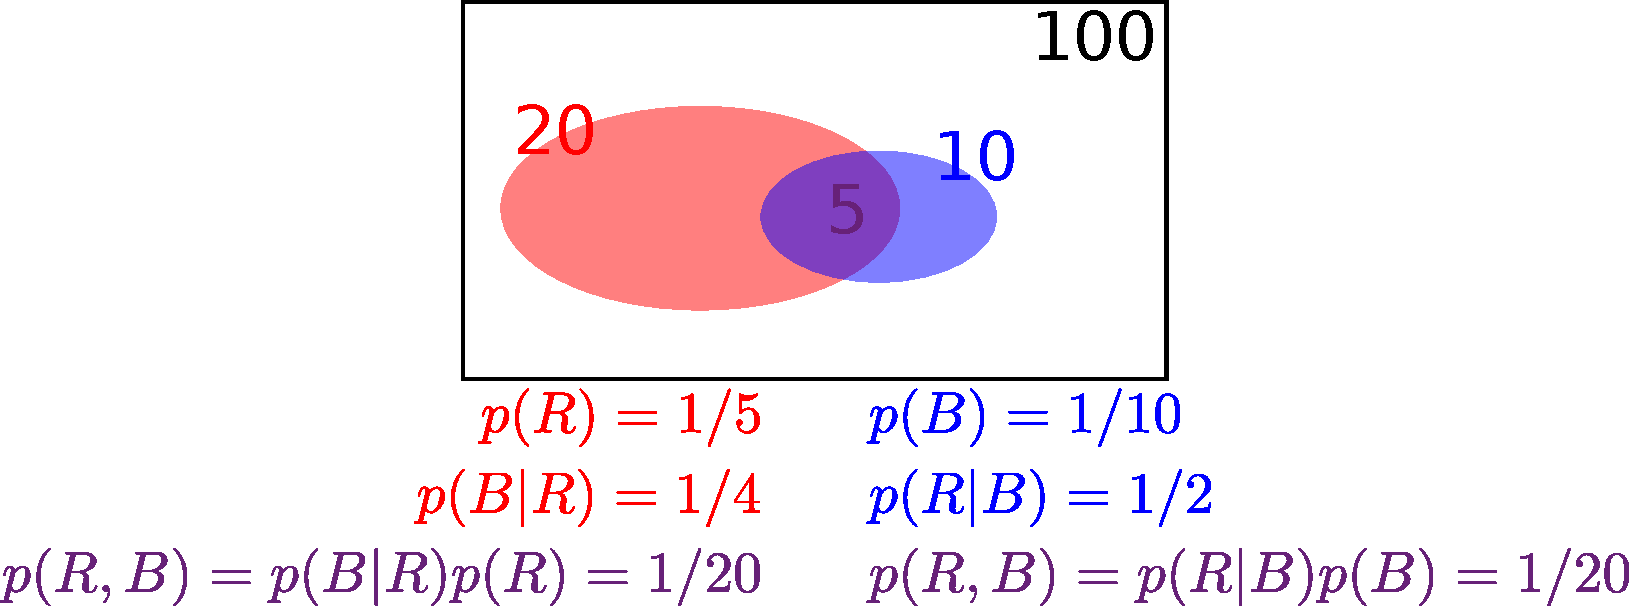
\includegraphics[width=1.35\textwidth]{figs/PRML_Bayes.pdf}
\end{figure}
\end{changemargin}
\end{frame}



\begin{frame}
\frametitle{Bayes Theorem}
\framesubtitle{Example from real life: Prosecutor's fallacy}
\mypagenum
\begin{itemize}
%\item Fallacy results from neglecting prior odds of a defendant being guilty
\item If someone is guilty, the probability of a DNA match is large, $p(D|g)$ is large
\begin{itemize}
\item convict?
\end{itemize}
\item Probability that a person is guilty if picked randomly from a large database is small, $p(g)$ is very small
\item Probability $p(D,g)=p(D|g)p(g)$ is not so large after all
\item So the prior information, $p(g)$ is important!
\end{itemize}
\end{frame}


%\begin{frame}
%\frametitle{Bayes Theorem}
%\framesubtitle{Example from real life: Berkson's paradox}
%\begin{itemize}
%\item $p(d)$ is small
%\item $p(m)$ is small
%\end{itemize}
%\end{frame}

%guest.imrani
%123


\begin{frame}
\frametitle{Bayes Theorem}
\framesubtitle{Relationship with time dynamic systems}
\mypagenum
\begin{itemize}
\item ${\color{red}p(x|z)} = \frac{{\color{blue}p(z|x)}{\color{darkgreen}p(x)}}{p(z)}$\\\vspace{0.2in}
{\color{red}Posterior distribution of states (our goal)}\\
{\color{darkgreen}Prior distribution of states (our belief)}\\
{\color{blue}Likelihood distribution (we can compute it)}\\
Observation probability (we won't need it!)\\\vspace{0.2in}
\item Now, what's the deal with recursion?
\end{itemize}
\end{frame}




%==========================
\subsection{\ \ \ \ Step 3. Recursion}
%==========================
\begin{frame}
\frametitle{Recursion}
\framesubtitle{}
\mypagenum
\begin{itemize}
\item In Bayes' theorem, we talked about 3 important probability distributions (posterior, prior, likelihood)
\item We want to compute the posterior distribution at every time instant
\item This is recursion, incremental updates, not batch mode
\end{itemize}
\end{frame}




\begin{frame}
\frametitle{Recursion}
\framesubtitle{}
\mypagenum
\begin{itemize}
\item We assume that our system and observation models are available in probabilistic form
\item The probabilistic state-space formulation and the requirement for updating of information on receipt of new measurements are ideally suited for the Bayesian approach
\begin{enumerate}
\item Prediction: predict states using model
\item Update: correction applied to prediction after observation arrives
\end{enumerate}
\end{itemize}
\end{frame}



\begin{frame}
\frametitle{Recursion}
\framesubtitle{a. Predict}
\mypagenum
\begin{table}
\begin{tabular}{|l|l|}\hline
$x_k$ & state at time $k$\\\hline
$Z_{k-1}$ &  all observations till time $k-1$\\\hline
\end{tabular}
\end{table}
\begin{figure}
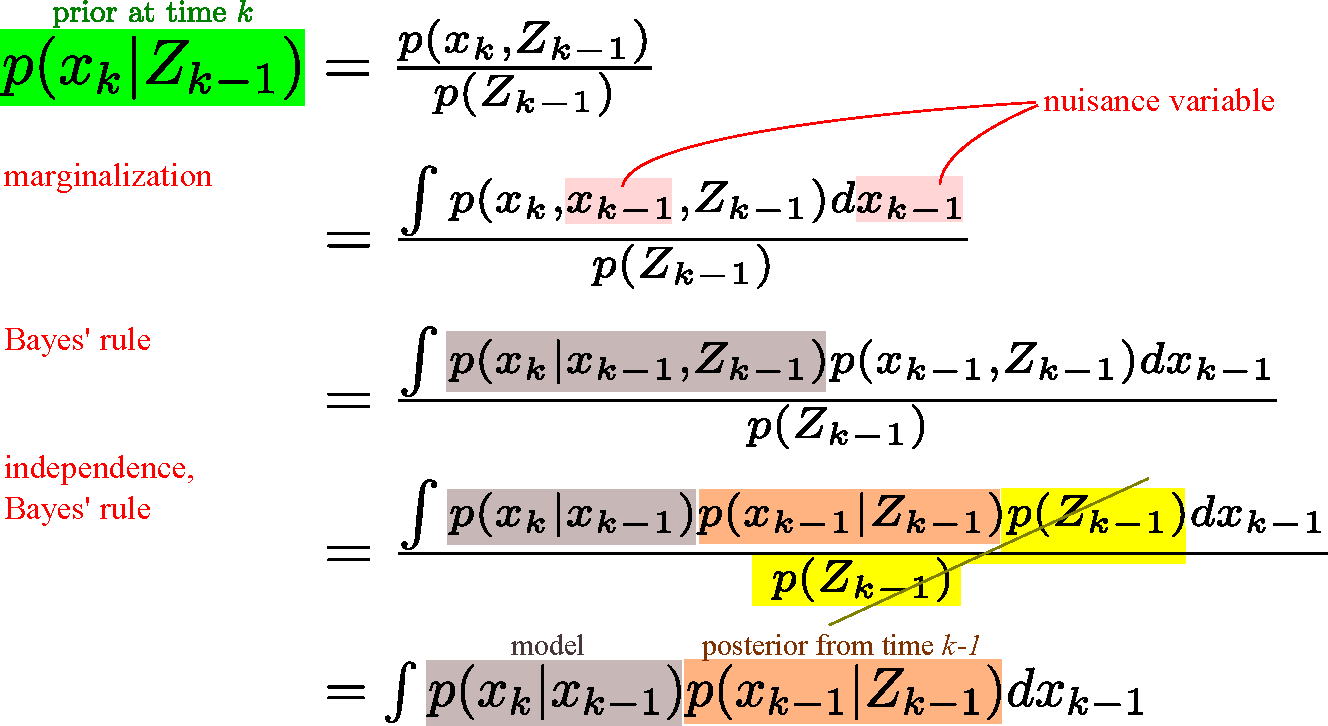
\includegraphics[width=0.8\textwidth]{figs/TRK_EQN_prediction.pdf}
\end{figure}
\end{frame}




\begin{frame}
\frametitle{Recursion}
\framesubtitle{b. Update}
\mypagenum
\begin{figure}
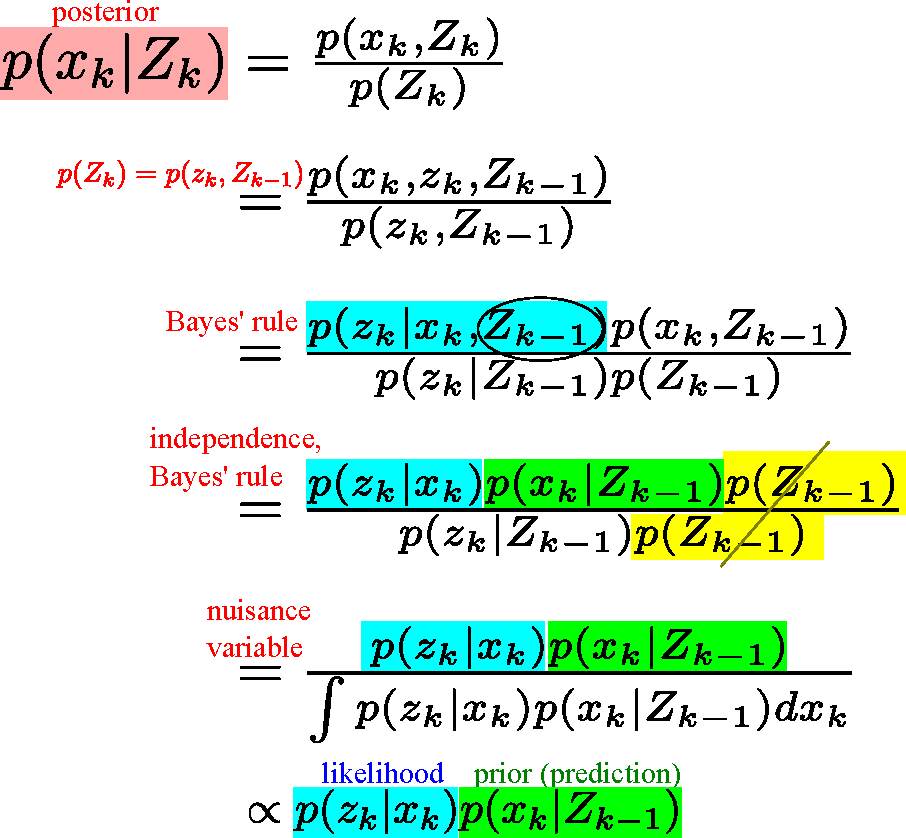
\includegraphics[height=0.8\textheight]{figs/TRK_EQN_update.pdf}
\end{figure}
\end{frame}



%==========================
\subsection{\ \ \ \ Step 4. Solutions}
%==========================
\begin{frame}
\frametitle{Solutions}
\framesubtitle{How to implement?}
\mypagenum
\begin{itemize}
\item The recursive propagation of the state density is only a conceptual solution in that in general, it cannot be determined analytically.
\item Solutions do exist in a restrictive set of cases, including the Kalman filter and grid-based filter
\begin{itemize}
\item State space is discrete and consists of finite number of states
\end{itemize}
\item In many situations of interest, the conditions of linearity and Gaussianity do not hold, and approximations are necessary.
\item Three approximate nonlinear Bayesian filters are the Extended Kalman Filter (EKF), approximate grid based methods and the particle filter
\end{itemize}
\end{frame}




\begin{frame}
\frametitle{Solutions}
\framesubtitle{Bigger picture}
\mypagenum
\begin{figure}
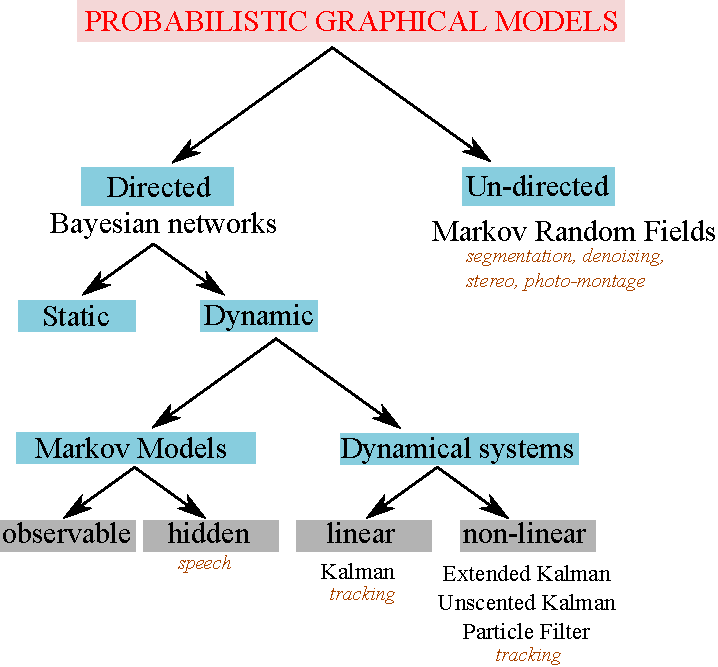
\includegraphics[width=0.65\textwidth]{figs/PRML_PGM_overview.pdf}
\end{figure}
\end{frame}

%------------------------------------------------------------
\subsubsection{\ \ \ \ \ \ \ \ HMM }
%------------------------------------------------------------
\begin{frame}
\frametitle{Solutions}
\framesubtitle{a. Hidden Markov Models}
\mypagenum
\begin{figure}
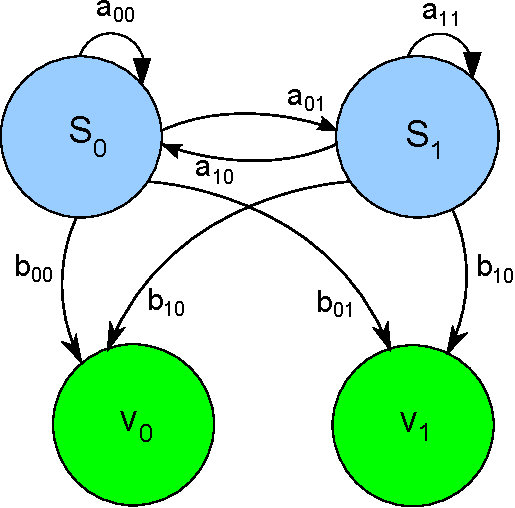
\includegraphics[height=0.3\textheight]{figs/HMM_flowDiagram.pdf}
\end{figure}
\begin{figure}
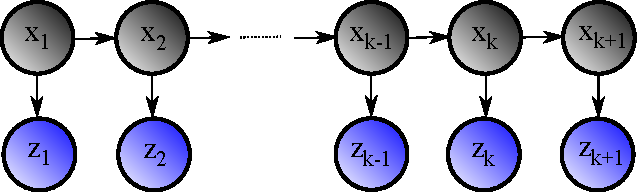
\includegraphics[width=1.0\textwidth]{figs/HMM_flowDiagram2.pdf}
\end{figure}
\end{frame}



\begin{frame}
\frametitle{Solutions}
\framesubtitle{b. Kalman Filter}
\mypagenum
\begin{figure}
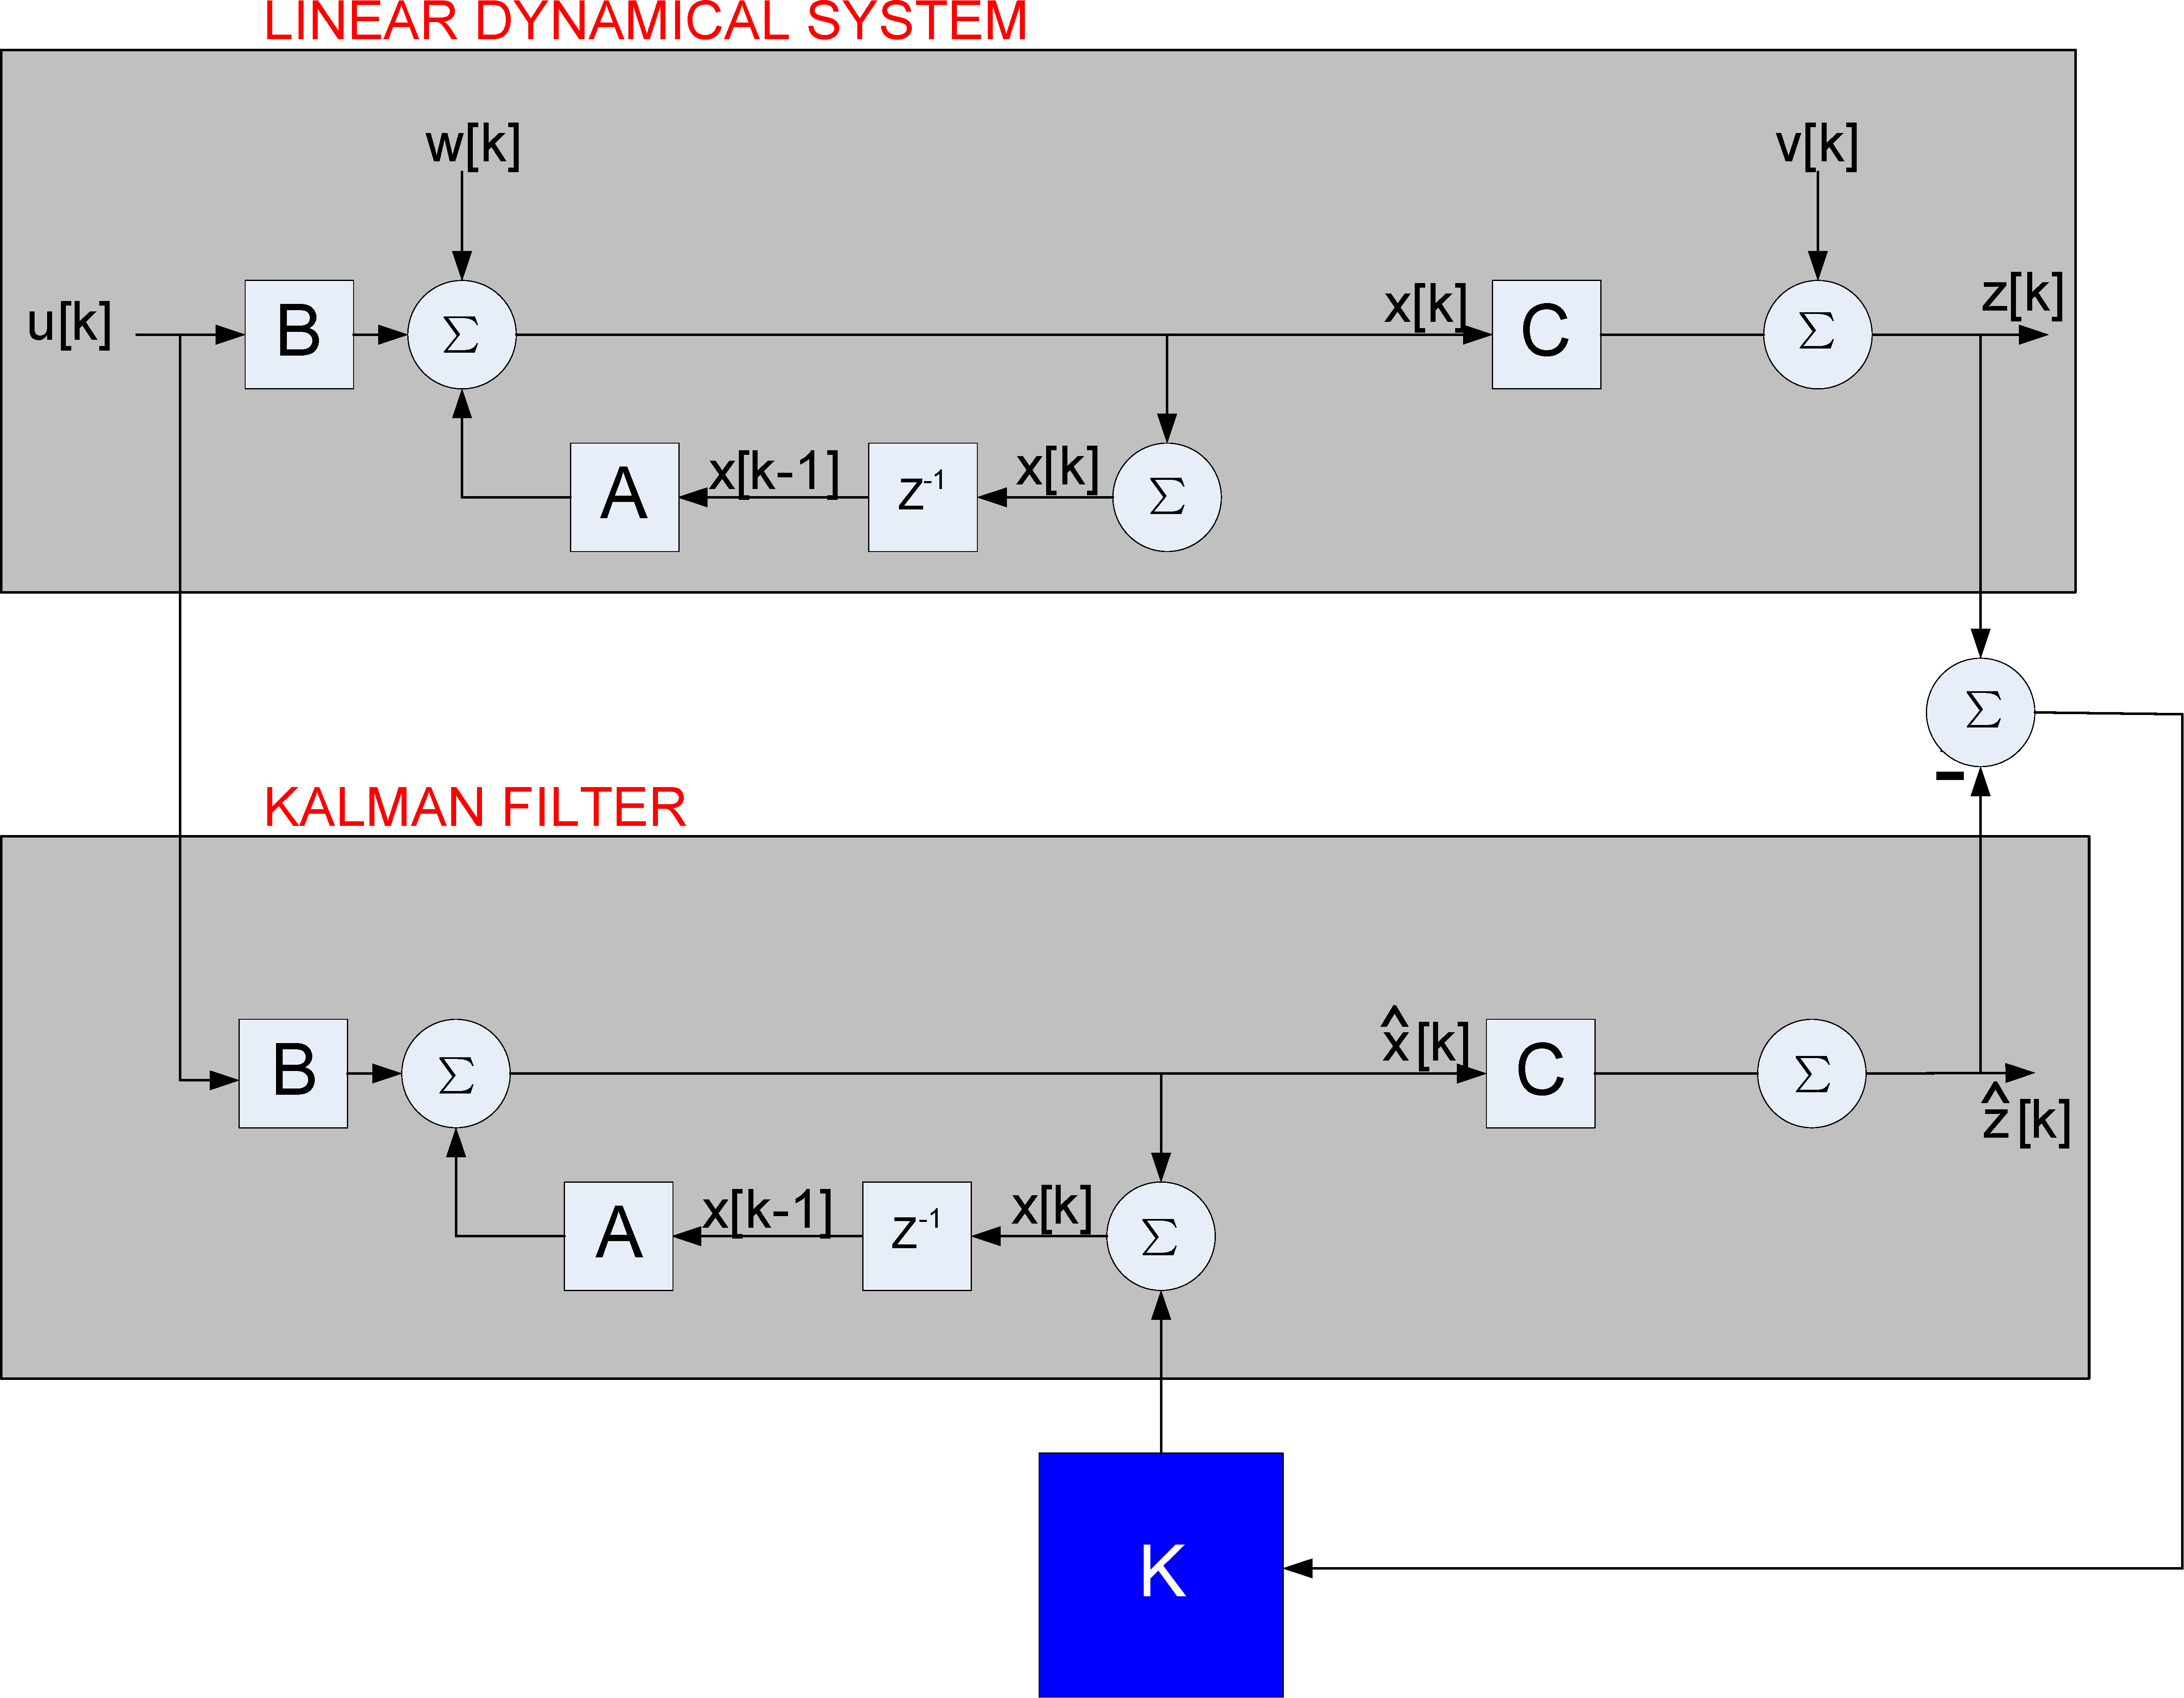
\includegraphics[width=0.8\textwidth]{figs/TRK_KalmanFilter_blockDiagram.pdf}
\end{figure}
\end{frame}




\begin{frame}
\frametitle{Solutions}
\framesubtitle{b. Kalman Filter}
\mypagenum
\begin{itemize}
\item {\color{red}Prior}
\begin{itemize}
\item Past information through time $k-1$
\item summarized approximately by a sufficient statistic in the form of a Gaussian posterior
\end{itemize}
\begin{equation*}
p(x_{k-1|k-1}|Z_{k-1})=\mathcal{N}  (\hat{x}_{k-1|k-1}, P_{k-1|k-1})
\end{equation*}
\item {\color{red}Prediction}
\begin{itemize}  
\item The state prediction is distributed as,
\begin{equation*}
p(x_{k|k-1}|Z_{k-1})=\mathcal{N}  (\hat{x}_{k|k-1}, P_{k|k-1})
\end{equation*}
\item The observation prediction is distributed as,
\begin{equation*}
p(z_{k|k-1})=\mathcal{N}  (\hat{z}_{k|k-1}, S_k)
\end{equation*}
\end{itemize}
\item {\color{red}Update}
\begin{itemize} 
\item innovation
\item Kalman gain
\item aposteriori state estimate and aposteriori covariance estimate
\end{itemize}
\end{itemize}
\end{frame}



\begin{frame}
\frametitle{Solutions}
\framesubtitle{b. Kalman Filter}
\mypagenum
\begin{figure}
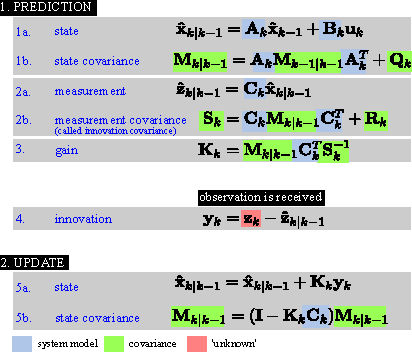
\includegraphics[width=0.72\textwidth]{figs/TRK_KalmanFilter_equations2.pdf}
\end{figure}
\end{frame}


%\begin{frame}\frametitle{Theory}\mypagenum
%	\begin{figure}
%		\includegraphics[width=0.7\textwidth]{figs/TRK_PDAF_probability_space.pdf}
%	\end{figure}
%\end{frame}

%\begin{frame}
%\frametitle{Tracking in clutter}
%\frametitle{MMSE, MMSE-MAP, MMSE-ML}
%\mypagenum
%\begin{figure}
%\includegraphics[width=0.9\textwidth]{figs/TRK_clutter_all.pdf}
%\end{figure}
%\end{frame}
%
%
%
%\begin{frame}
%\frametitle{Tracking in clutter}
%\framesubtitle{MMSE}
%\mypagenum
%	\begin{figure}
%		\includegraphics[width=1.0\textwidth]{figs/TRK_clutter_MMSE.pdf}
%	\end{figure}
%\end{frame}






%------------------------------------------------------------
\subsubsection{\ \ \ \ \ \ \ \ PDAF }
%------------------------------------------------------------
\begin{frame}
\frametitle{Solutions}
\framesubtitle{c. PDAF: Extension of Kalman Filter}
\mypagenum
{\color{red} Probabilistic Data Association Filter}
\begin{itemize}
\item Computationally efficient 
\item Data association
\item Single targets in clutter, high false alarm rate
\item Extension of Kalman filter
\begin{itemize}
\item Primary difference: computation of innovations
\item Calculates association probabilities to the target for each validated measurement
\end{itemize}
\end{itemize}
\end{frame}



%\begin{frame}\frametitle{Other solutions}\mypagenum
%	\begin{itemize}
%		\item Standard filter: pick one of them, e.g. nearest neighbor (possibly incorrect)
%		\item Track split: one track for every possible measurement (computationally expensive)
%	\end{itemize}
%\end{frame}




\begin{frame}
\frametitle{Solutions}
\framesubtitle{c. PDAF: Extension of Kalman Filter}
\mypagenum
Assumptions:
\begin{enumerate}
\item  {\color{red}{Number of targets}}
\begin{itemize}
\item Single target tracking
\end{itemize}
\item {\color{red}{False alarms}}
\begin{itemize} 
\item At most, one of the validated measurements can be target originated	
\item Remaining measurements
\begin{itemize}
\item incorrect, i.e., false alarms
\item i.i.d
\item parametric form: Poisson distribution with known spatial density $\lambda$
\item non-parametric form: uniform spatial distribution
\end{itemize}
\end{itemize}
\end{enumerate}
\end{frame}




%\begin{frame}
%\frametitle{PDAF}
%\framesubtitle{assumptions (cont.)}
%\mypagenum
%	\begin{enumerate}\setcounter{enumi}{2}
%		\item {\color{red}{Target detection}}
%		\begin{itemize} 
%			\item Known probability, $P_D$
%		\end{itemize}
%		%\item Innovation of correct return normally distributed
%		\item {\color{red}{Prior}}
%		\begin{itemize} 
%			\item Density of the state conditioned on the past observations is a Gaussian distribution,		
%		\end{itemize}
%		\begin{equation*}
%			p(\mathbf{x}_{k-1}|Z^{k-1}) = \mathcal{N}  (  \hat{\mathbf{x}}_{k-1|k-1}, \mathbf{P}_{k-1|k-1})
%		\end{equation*}
%	\end{enumerate}
%\end{frame}



\begin{frame}
\frametitle{Solutions}
\framesubtitle{c. PDAF: Extension of Kalman Filter}
\footnote{ \tiny Bar-shalom, 2009}
\mypagenum	
\begin{figure}
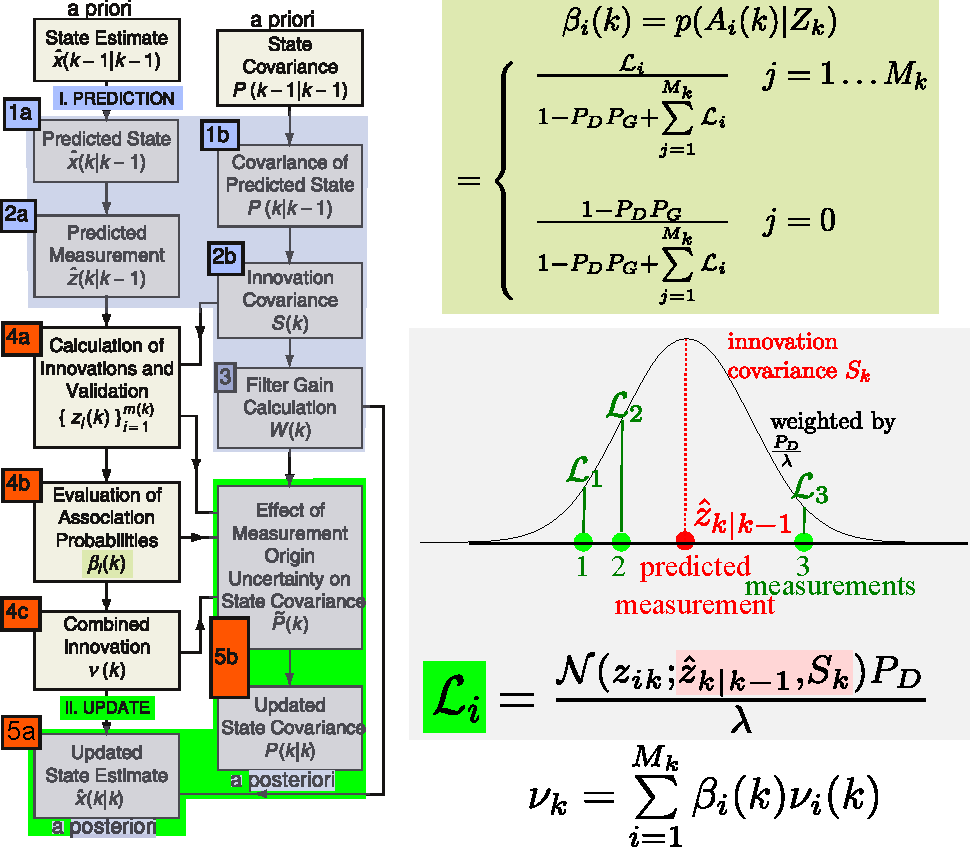
\includegraphics[height=0.7\textheight]{figs/TRK_PDAF_flowDiagram.pdf}
\end{figure}	
\end{frame}





%\begin{frame}
%\frametitle{PDAF}
%\framesubtitle{innovations, step 1}
%\mypagenum
%	{\color{red}Measurement validation}
%	\begin{itemize} 
%		\item only measurements inside a validation gate are accepted. 
%		\item $P_G$: If the true measurement is detected,  $P_G$ is the probability that it is in the gate
%	\end{itemize}
%\end{frame}
%
%
%
%
%
%\begin{frame}
%\frametitle{PDAF}
%\framesubtitle{innovations, step 2}
%\mypagenum
%	\begin{itemize}
%		\item {\color{red} Association events, $A_i$}
%		\begin{itemize}
%			\item mutually exclusive and exhaustive
%			\item Example of three measurements
%			\begin{itemize}
%				\item $z_1$ originated from target, $z_2$ and $z_3$ are spurious
%				\item $z_2$ originated from target, $z_1$ and $z_3$ are spurious
%				\item $z_3$ originated from target, $z_1$ and $z_2$ are spurious
%				\item All are spurious
%			\end{itemize}
%		\end{itemize}
%		\item {\color{red} Association probabilities, $\beta_i$}
%		\begin{itemize}
%			\item $\beta_i$ the aposterior probability that the $i$-th return originated from the object in track
%			\item$\beta_0$ is the probability that none of the measurements are correct
%		\end{itemize}
%	\end{itemize}
%\end{frame}
%
%
%
%
%\begin{frame}
%\frametitle{PDAF}
%\framesubtitle{innovations, step 2 (cont.)}
%\mypagenum
%	Computing the association probabilities, $\beta_{ik}$,
%	\begin{align*}
%		\beta_{ik} &\triangleq p(A_{ik}|Z_k)\\
%				&=	\left\{ 
%						\begin{array}{cc}
%							\frac{\mathcal{L}_i}{1-P_DP_G + \sum\limits_{j=1}^{j=M_k} \mathcal{L}_i}  & j=1 \ldots M_k\\ \\
%							\frac{1-P_DP_G}{1-P_DP_G + \sum\limits_{j=1}^{j=M_k} \mathcal{L}_i} & j=0
%						\end{array} 
%					\right. \\
%		\mathcal{L}_i&= \frac{\mathcal{N}  (z_{ik};  \hat{z}_{k|k-1}, S_k)P_D}{\lambda}
%	\end{align*}
%\end{frame}
%
%
%
%
%\begin{frame}
%\frametitle{PDAF}
%\framesubtitle{innovations, step 2 (cont.)}
%\mypagenum	
%	\begin{align*}
%		\mathcal{L}_i&= \frac{\mathcal{N}  (z_{ik};  \hat{z}_{k|k-1}, S_k)P_D}{\lambda}
%	\end{align*}
%	\begin{itemize}
%		\item Likelihood $L_i$ is centered around the predicted observation
%		\begin{itemize}
%			\item Far away clutter has exponentially lower weight
%		\end{itemize}
%	\end{itemize}
%\end{frame}
%
%
%
%
%\begin{frame}
%\frametitle{PDAF}
%\framesubtitle{innovations, step 3}
%\mypagenum
%	{\color{red} Innovations, $\nu_{ik}$}
%	\begin{itemize}
%		\item $\mathbf{\nu}_{ik}$  for each measurement $\mathbf{z}_{ik}$ are computed using the conditional mean of the observations $\hat{\mathbf{z}}(k|k-1)$:
%		\begin{equation*}
%			\nu_{ik}  \triangleq \mathbf{z}_{ik} - \hat{\mathbf{z}}(k|k-1) 
%		\end{equation*}
%	\end{itemize}
%\end{frame}
%
%
%
%\begin{frame}
%\frametitle{PDAF}
%\framesubtitle{innovations, step 4}
%\mypagenum
%	{\color{red} Combined innovation, $y_k$}
%	\begin{itemize}
%		\item $\mathbf{\nu}_{ik}$ and $\beta_{ik}$ for each target are combined to form a combined innovation:  
%		\begin{equation*}
%			y_k  \triangleq \sum_{i=1}^{M_k} \beta_{ik}\nu_{ik}
%		\end{equation*}
%	\item If there is only one measurement, i.e., $M_k=1$, PDAF becomes equivalent to the Kalman Filter
%	\end{itemize}
%\end{frame}
%
%
%
%
%\begin{frame}
%\frametitle{PDAF}
%\framesubtitle{covariance update}
%\mypagenum
%	\begin{align*}
%		\mathbf{P}_{k|k-1} =
%		&\beta_{0k}\mathbf{P}_{k|k-1} +\\
%		&\left[1-\beta_{0k}\right]\left[\mathbf{P}_{k|k-1}-\mathbf{K}_k\mathbf{S}_k\mathbf{K}_k'\right] +\\
%		&\mathbf{K}_k\left[\sum\limits_{i=1}^{m_k}\beta_{ik}y_{ik}y_{ik}'-y_{k}y_{k}'\right]\mathbf{K}_k' 
%	\end{align*}
%\end{frame}
%
%
%
%
%\begin{frame}
%\frametitle{PDAF}
%\framesubtitle{limitations}
%\mypagenum
%	\begin{itemize}
%		\item The PDAF algorithm makes an assumption that a single target is being tracked.  
%		\item Additional targets handled with multiple copies of the filter.  
%		\item However, in such cases, measurements from interfering targets do not behave like a Poisson process.  
%		\item Solution: JPDAF
%	\end{itemize}
%\end{frame}



\begin{frame}
\frametitle{Solutions}
\framesubtitle{c. PDAF: Extension of Kalman Filter}
\mypagenum
	PDAF + multiple model Kalman Filters \tiny{\footnote{Bar-Shalom et al., 2009}}:
	\begin{figure}
		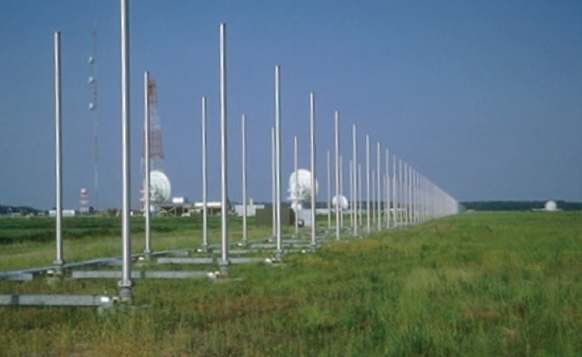
\includegraphics[width=0.8\textwidth]{figs/TRK_PDAF_example_US_Navy_ROTHR.jpg}
		\caption {US Navy ROHR (Relocatable Over the Horizon Radar) for long-range surveillance for drug interdiction against aircraft and ships}
	\end{figure}
\end{frame}

%------------------------------------------------------------
\subsubsection{\ \ \ \ \ \ \ \ JPDAF }
%------------------------------------------------------------
\begin{frame}
\frametitle{Solutions}
\framesubtitle{d. JPDAF: Extension of Kalman Filter}
\mypagenum
	{\color{red} Joint Probabilistic Data Association Filter}
	\begin{itemize}
		\item Extension of PDAF to multi-target tracking	
			\begin{itemize}
				\item Only difference: computation of association probabilities, $\beta_{ik}$
			\end{itemize}
		\item Handles multiple targets by considering all measurements for all targets.  
		\item Probability density of each candidate measurement
			\begin{itemize}
				\item Based on all close-by targets
			\end{itemize}
	\end{itemize}
\end{frame}




\begin{frame}
\frametitle{Solutions}
\framesubtitle{d. JPDAF: Extension of Kalman Filter}
\mypagenum 	
Association probabilities
	\begin{figure}
		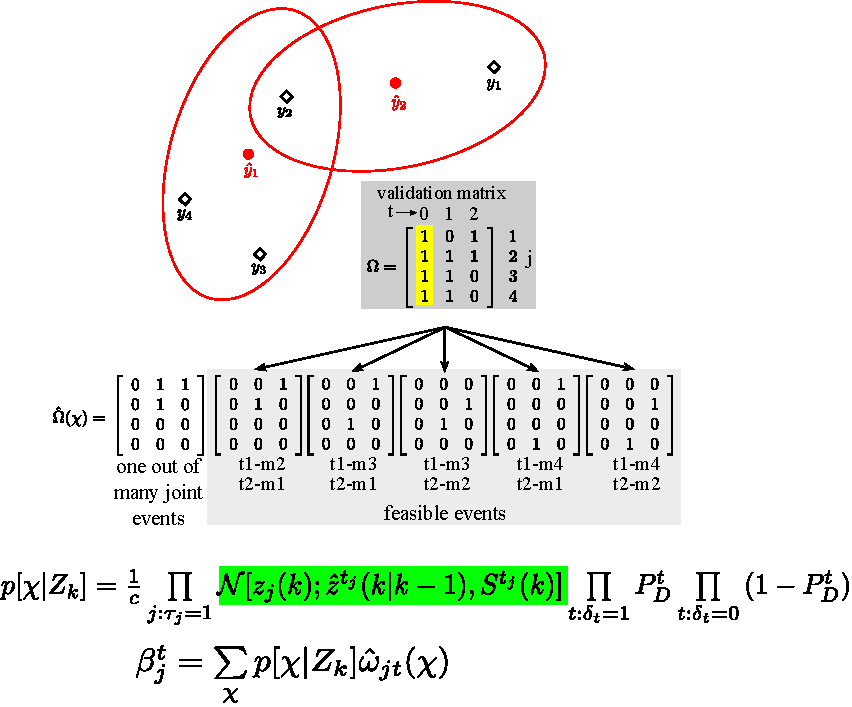
\includegraphics[height=0.80\textheight]{figs/TRK_JPDAF_twoTargetScenario.pdf}
	\end{figure}	
\end{frame}

%\begin{frame}\frametitle{JPDAF}\mypagenum
%	\begin{enumerate}
%		\item Measurement validation: The measurements are not gated, and all measurements are considered for every target.
%	\end{enumerate}
%\end{frame}		




%\begin{frame}
%\frametitle{JPDAF}
%\framesubtitle{steps}
%\mypagenum
%	\begin{itemize}%\setcounter{enumi}{2}
%		\item Joint association probabilities for joint association events
%		\item $A_{jt}(k)$ is the event that measurement $j$ at time $k$ originated from target $t$
%		\begin{equation*}
%			A(k) = \bigcap_j A_{jt}(k)
%		\end{equation*}
%		\item The probability of $A(k)$ given all measurements $Z_k$ is given by
%		\begin{align*}
%			\small
%			p[A(k)|Z^k] 	&= \frac{1}{c} \prod_j \{ \mathcal{N} [z_j(k); \\ 
%						&\hat{z}^{t_j}(k|k-1), S^{t_j}(k)] \}^{\tau_j	}\\
%						& \prod_t {P^t_D}^{\delta_t}{(1-P_D)}^{1-\delta_t}
%		\end{align*}
%	\end{itemize}
%\end{frame}





%\begin{frame}
%\frametitle{JPDAF}
%\framesubtitle{steps (cont.)}
%\mypagenum
%	\begin{itemize}	
%		\item A combined innovation is computed using the joint association probabilities using
%		\begin{align*}
%			\beta_{j}(k) &\triangleq p[A_{jt}(k)|Z_k]  \notag\\
%			&= \sum_{A:A_{jt} \in A} p[A(k)|Z_k]
%		\end{align*}
%	\end{itemize}
%\end{frame}




\begin{frame}
\frametitle{Solutions}
\framesubtitle{d. JPDAF: Extension of Kalman Filter}
\mypagenum
	Nearest neighbor JPDAF + EKF:
	\begin{columns}
		\begin{column}{1.0in}
			\begin{figure}
			{
				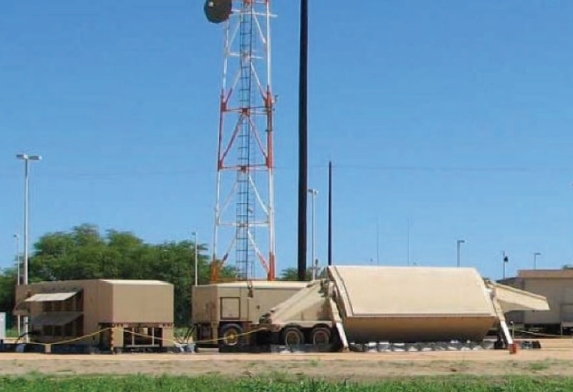
\includegraphics[width=1.0in]{figs/TRK_JPDAF_example_THAAD.jpg}
				\caption {THAAD, \\Theater High Altitude Area Defense)}
			}
			\end{figure}
		\end{column}
		\begin{column}{1.0in}
			\begin{figure}
			{
				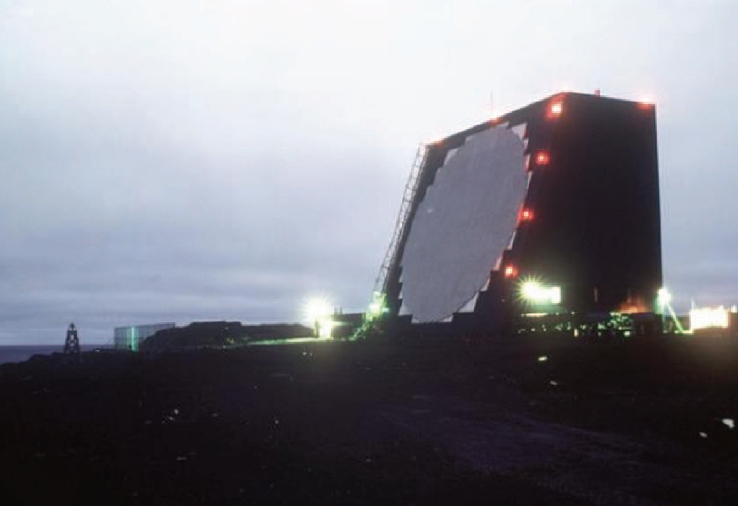
\includegraphics[width=1.0in]{figs/TRK_JPDAF_example_Cobra.jpg}
				\caption {Cobra Dane,\\long-range surveillance against ICBMs}
			}
			\end{figure}
		\end{column}
		\begin{column}{1.0in}
			\begin{figure}
			{
				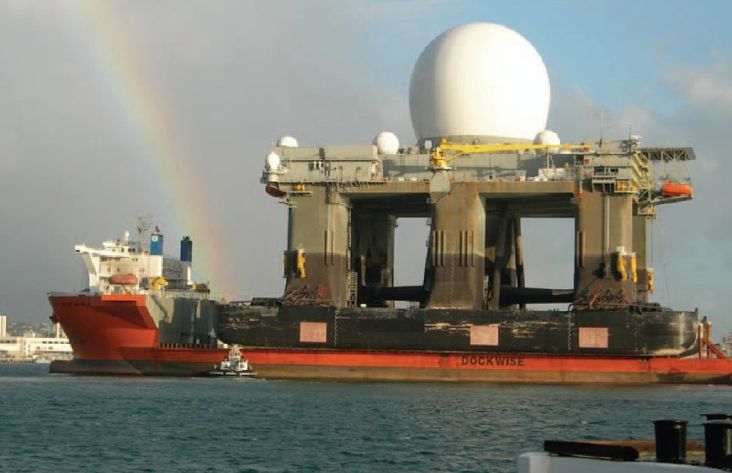
\includegraphics[width=1.0in]{figs/TRK_JPDAF_example_SBX.jpg}
				\caption {SBX,\\long-range surveillance against ICBMs}
			}
			\end{figure}
		\end{column}
	\end{columns}
\end{frame}



%------------------------------------------------------------
\subsubsection{\ \ \ \ \ \ \ \ MHT }
%------------------------------------------------------------
\begin{frame}
\frametitle{Solutions}
\framesubtitle{e. Multi-hypothesis tracker}
\mypagenum
	\begin{enumerate}
	\item {\color{red}Clustering}
		\begin{itemize}
			\item A new measurement is associated with a cluster if it falls within the validation region of any target within the cluster
		\end{itemize}
	\item {\color{red}Hypothesis Generation}
		\begin{itemize} 
			\item New hypotheses are generated for the measurements associated with each cluster
			\item The probability of each hypothesis is calculated
			\item Target estimates are then updated
		\end{itemize}
	\item {\color{red}Reduction}
		\begin{itemize}
			\item In this step, hypotheses are combined or eliminated
		\end{itemize}
	\item {\color{red}Simplify hypothesis matrix}
		\begin{itemize}
			\item Targets that are uniquely associated are removed from the hypothesis matrix
		\end{itemize}
	\end{enumerate}
\end{frame}




\begin{frame}
\frametitle{Solutions}
\framesubtitle{e. Multi-hypothesis tracker}
\mypagenum
	MHT + EKF:
	\begin{figure}
		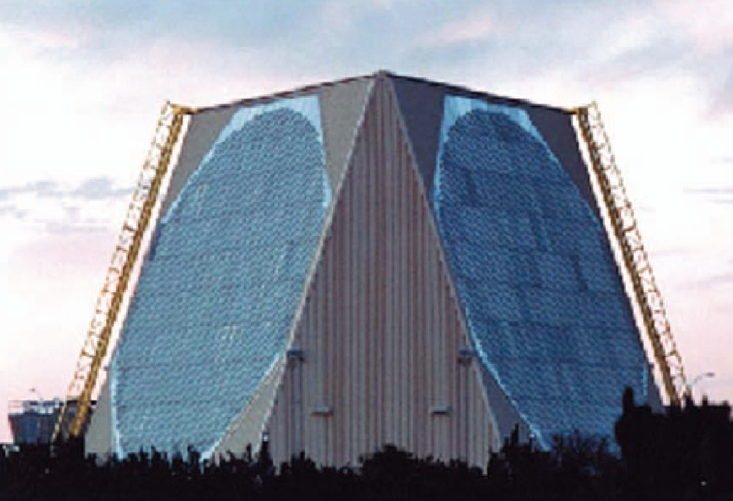
\includegraphics[width=0.7\textwidth]{figs/TRK_MHT_example_UEWR.jpg}
		\caption {UEWR, Upgraded Early Warning Radar, long-range surveillance against ICBMs}
	\end{figure}
\end{frame}



%
%\begin{frame}
%\frametitle{Predict and Update}
%\framesubtitle{Tracking}
%Estimate and maintain {\color{red}target state} over {\color{red}time}
%\begin{figure}
%\includegraphics[width=1.0\textwidth]{thesis/TRK_overviewDiagram.pdf}
%\end{figure}
%\end{frame}











\begin{frame}
\frametitle{Solutions}
\framesubtitle{f. Particle filter}
\mypagenum
\begin{itemize}
\item All densities are modeled using samples
\item Two step process, predict, and then update using resampling
\end{itemize}
\end{frame}




\begin{frame}
\frametitle{Solutions}
\framesubtitle{f. Particle filter}
\mypagenum
\footnote{\tiny http://lia.deis.unibo.it/research/SOMA/MobilityPrediction/filters.shtml}
\begin{figure}
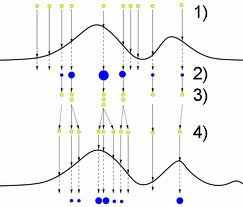
\includegraphics[width=0.6\textwidth]{figs/PRML_update.jpg}
\end{figure}
\end{frame}



\begin{frame}
\frametitle{Solutions}
\framesubtitle{f. Particle filter}
\mypagenum
\footnote{\tiny Smith Gelfand, Bayesian Statistics Without Tears, A Sampling Resampling Perspective, 1992}
\begin{itemize}
\item There is an essential duality between a sample and the density (distribution) from which it is generated
\begin{itemize}
\item The density generates the sample
\item Conversely, given a sample, we can approximately recreate the density
\end{itemize}
\item In terms of densities, the inference process is encapsulated in the updating of the prior density $p(x)$ to the posterior density $p(x|z)$ through the medium of the likelihood function $p(z|x)$
\item In terms of samples, this corresponds to the updating of a sample from $p(x)$ to a sample from $p(x|z)$ through the likelihood function $p(z|x)$
\end{itemize}
\end{frame}


\begin{frame}
\frametitle{Solutions}
\framesubtitle{f. Particle filter}
\mypagenum
\footnote{\tiny Arulampalam et al., A tutorial on particle filters for online nonlinear non-Gaussian Bayesian Tracking, 2002}
\begin{itemize}
\item In many application areas, elements of nonlinearity and non-Gaussianity need to be included to accurately model the underlying dynamics of a physical system
\item Moreover, it is typically crucial to process data on-line as it arrives
\item Particle filters are Sequential Monte Carlo (SMC) methods based on point-mass (or "particle") representations of probability densities which can be applied to any state-space model
\item The particle filter generalizes the Kalman filter
\item The algorithm used is Sequential Importance Sampling (SIS)
\end{itemize}
\end{frame}





%\begin{frame}
%\frametitle{Solutions}
%\framesubtitle{c. Particle filter}
%\begin{itemize}
%\item Many problems in science require estimation of the state of a system that changes over time using a sequence of noisy measurements made on the system
%\item In tracking problems, the state vector could be related to the kinematics of the target
%\item In economics, it could be related to monetary flow, interest rates, inflation, etc.
%\end{itemize}
%\end{frame}





%\begin{frame}
%\frametitle{Solutions}
%\framesubtitle{c. Particle filter}
%\begin{itemize}
%\item In the Bayesian approach to dynamic state estimation, one attempts to construct the posterior probability density function (pdf) of the state based on all available information, including the set of received measurements
%\item Since this pdf embodies all statistical information, 
%\end{itemize}
%\end{frame}
%
%
%
%
%
%\begin{frame}
%\frametitle{Solutions}
%\framesubtitle{c. Particle filter}
%\begin{itemize}
%\item The probabilistic state-space formulation and the requirement for updating the information on receipt of new measurements are ideally suited for the Bayesian approach
%\item In the Bayesian approach to dynamic state-estimation, one attempts to construct the posterior pdf of the state based on all available information, including the set of received measurements
%\item For many problems, an estimate is required every time a measurement is received.  In this case, a recursive filter is a convenient solution.  A recursive filtering approach means that received data can be processed sequentially rather than as a batch so that it is not necessary to store the complete data set nor to reprocess existing data if a new measurement becomes available
%\end{itemize}
%\end{frame}


%\begin{frame}
%\frametitle{Solutions}
%\framesubtitle{c. Particle filter}
%\begin{itemize}
%\item Such a filter consists of essentially 2 stages: prediction update
%\item The prediction stage uses the system model to predict the state pdf forward from one measurement time to the next
%\item Since the state is usually subject to unknown disturbances (modeled as random noise), prediction generally translates, deforms, and spreads the state pdf
%\item The update operation uses the latest measurement to modify the prediction pdf
%\item This is achieved using Bayes theorem, which is the mechanism for updating knowledge about the target state in the light of extra information from new data
%\end{itemize}
%\end{frame}












%\begin{frame}
%\frametitle{Solutions}
%\framesubtitle{c. Particle filter}
%\scriptsize
%\begin{figure}[t]
%\centering
%\subfigure[Reference (uniform) density and test PDF.]{\includegraphics[width=0.3\textwidth]{thesis/particle_filter_pdfs.pdf}}
%\subfigure[Comparing CDFs.]{\includegraphics[width=0.38\textwidth]{thesis/particle_filter_resampling.pdf}}
%\subfigure[Particles 4, 7 and 9 are picked repeatedly.]{\includegraphics[width=0.3\textwidth]{thesis/particle_filter_particles.pdf}}
%\caption{Particle filter, resampling.}
%\label{fig:particle_filter_resampling}
%\end{figure}
%\end{frame}










%%####################################################################################################
%\section{Examples}
%%####################################################################################################
%\begin{frame}
%\frametitle{Examples}
%\framesubtitle{}
%Let's look at a 1D and 2D example.
%\end{frame}
%
%%==========================
%\subsection{\ \ \ \ 1D}
%%==========================
%\begin{frame}
%\frametitle{Example}
%\framesubtitle{1D tracking with particle filter}
%\begin{figure}
%\includegraphics[width=0.8\textwidth]{thesis/TRK_ParticleFilter_multimodalPDF.pdf}
%\end{figure}	
%\end{frame}
%
%
%
%%==========================
%\subsection{\ \ \ \ 2D}
%%==========================
%\begin{frame}
%\frametitle{Example}
%\framesubtitle{2D tracking with particle filter}
%Use random affine deformation to model motion
%\begin{itemize}
%\item Perturb affine parameters
%\item For each affine set, 
%\begin{itemize}
%\item apply forward affine transform on zero-centered canonical grid 
%\item bilinear interpolation to extract ROI, one per affine set, as shown below
%\begin{figure}[t]
%\centering
%\includegraphics[width=0.32\textwidth]{thesis/affineCandidates.pdf}
%\label{Fig:affine_candidates}
%\end{figure}
%\end{itemize}
%\item For set corresponding to least reconstruction error, apply forward affine transform to $(\mathbf{x, y})$ and compare with ground truth to get track error
%\end{itemize}
%\end{frame}
%
%
%
%\begin{frame}
%\frametitle{Example}
%\framesubtitle{2D tracking with particle filter}
%Density of grid points is greater in the horizontal direction.
%\begin{figure}[t]
%\centering
%\fbox{\includegraphics[width=0.8\textwidth]{thesis/dataset_Dudek_00001_forwardAffine.pdf}}
%\end{figure}
%\end{frame}


%####################################################################################################
\section{Conclusion}
%####################################################################################################
\begin{frame}
\frametitle{Conclusion}
\mypagenum
\framesubtitle{}
\begin{itemize}
\item There are many solutions to the Bayesian recursion equations
\item The Kalman Filter is optimal if these equations are linear and the models are Gaussian
\end{itemize}
\end{frame}





%####################################################################################################
\end{document}
%####################################################################################################

